
\section{V - MNIST}
\begin{frame}{V - Reconnaissance d'image}
	\begin{block}{Problématique : Reconnaissance des chiffres écrits à la main}
		Images de taille $28 \times 28$ pixels en noir et blanc : \\
		\quad - 60 000 images pour l'entrainement. \\
		\quad - 10 000 autres pour la vérification.
	\end{block}
	\begin{figure}
		\centering
		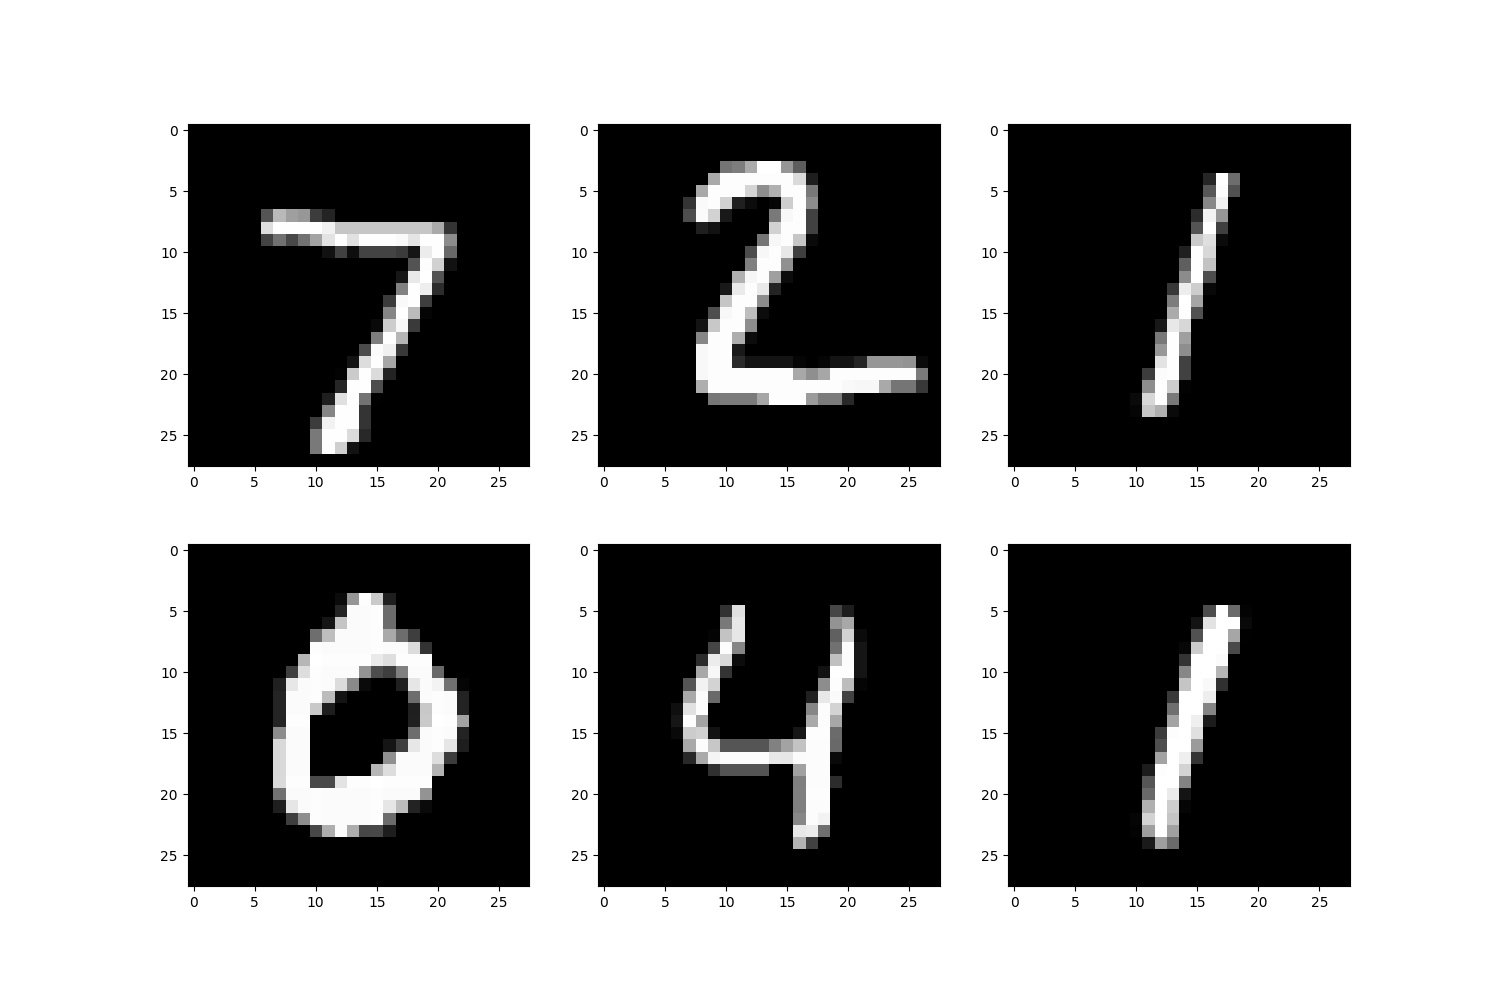
\includegraphics[width=150px]{1-mnist.jpg}
		\caption{Exemple d'images}
	\end{figure}
\end{frame}


\begin{frame}{V - Apprentissage d'un problème de classification}
	On prend un réseau de neurones avec $28 \times 28 = 784$ entrées, et 10 sorties. \\
	\begin{block}{Softmax}
		La fonction d'activation softmax permet de normaliser en probabilités les sorties : \\
		• $p_i = \frac{exp(a_i)}{\sum_{k=1}^{n}exp(a_k)}$ la probabilité de la sortie $a_i$ \\
		• $\dfrac{\partial p_i}{\partial a_j} = p_i\times(\delta_{ij}-p_j)$ \\
	\end{block}
	\begin{block}{Cross-entropy}
		La fonction coût des problèmes de classification est Cross-entropy : \\
		• $L\ \ \ = -\sum_{k=1}^{n}y_ilog(p_i)$ avec $y_i$ la sortie attendue \\
		• $\dfrac{\partial L}{\partial a_i} = p_i - y_i$
	\end{block}
\end{frame}


\begin{frame}{V - Softmax}
	\begin{figure}
		\centering
		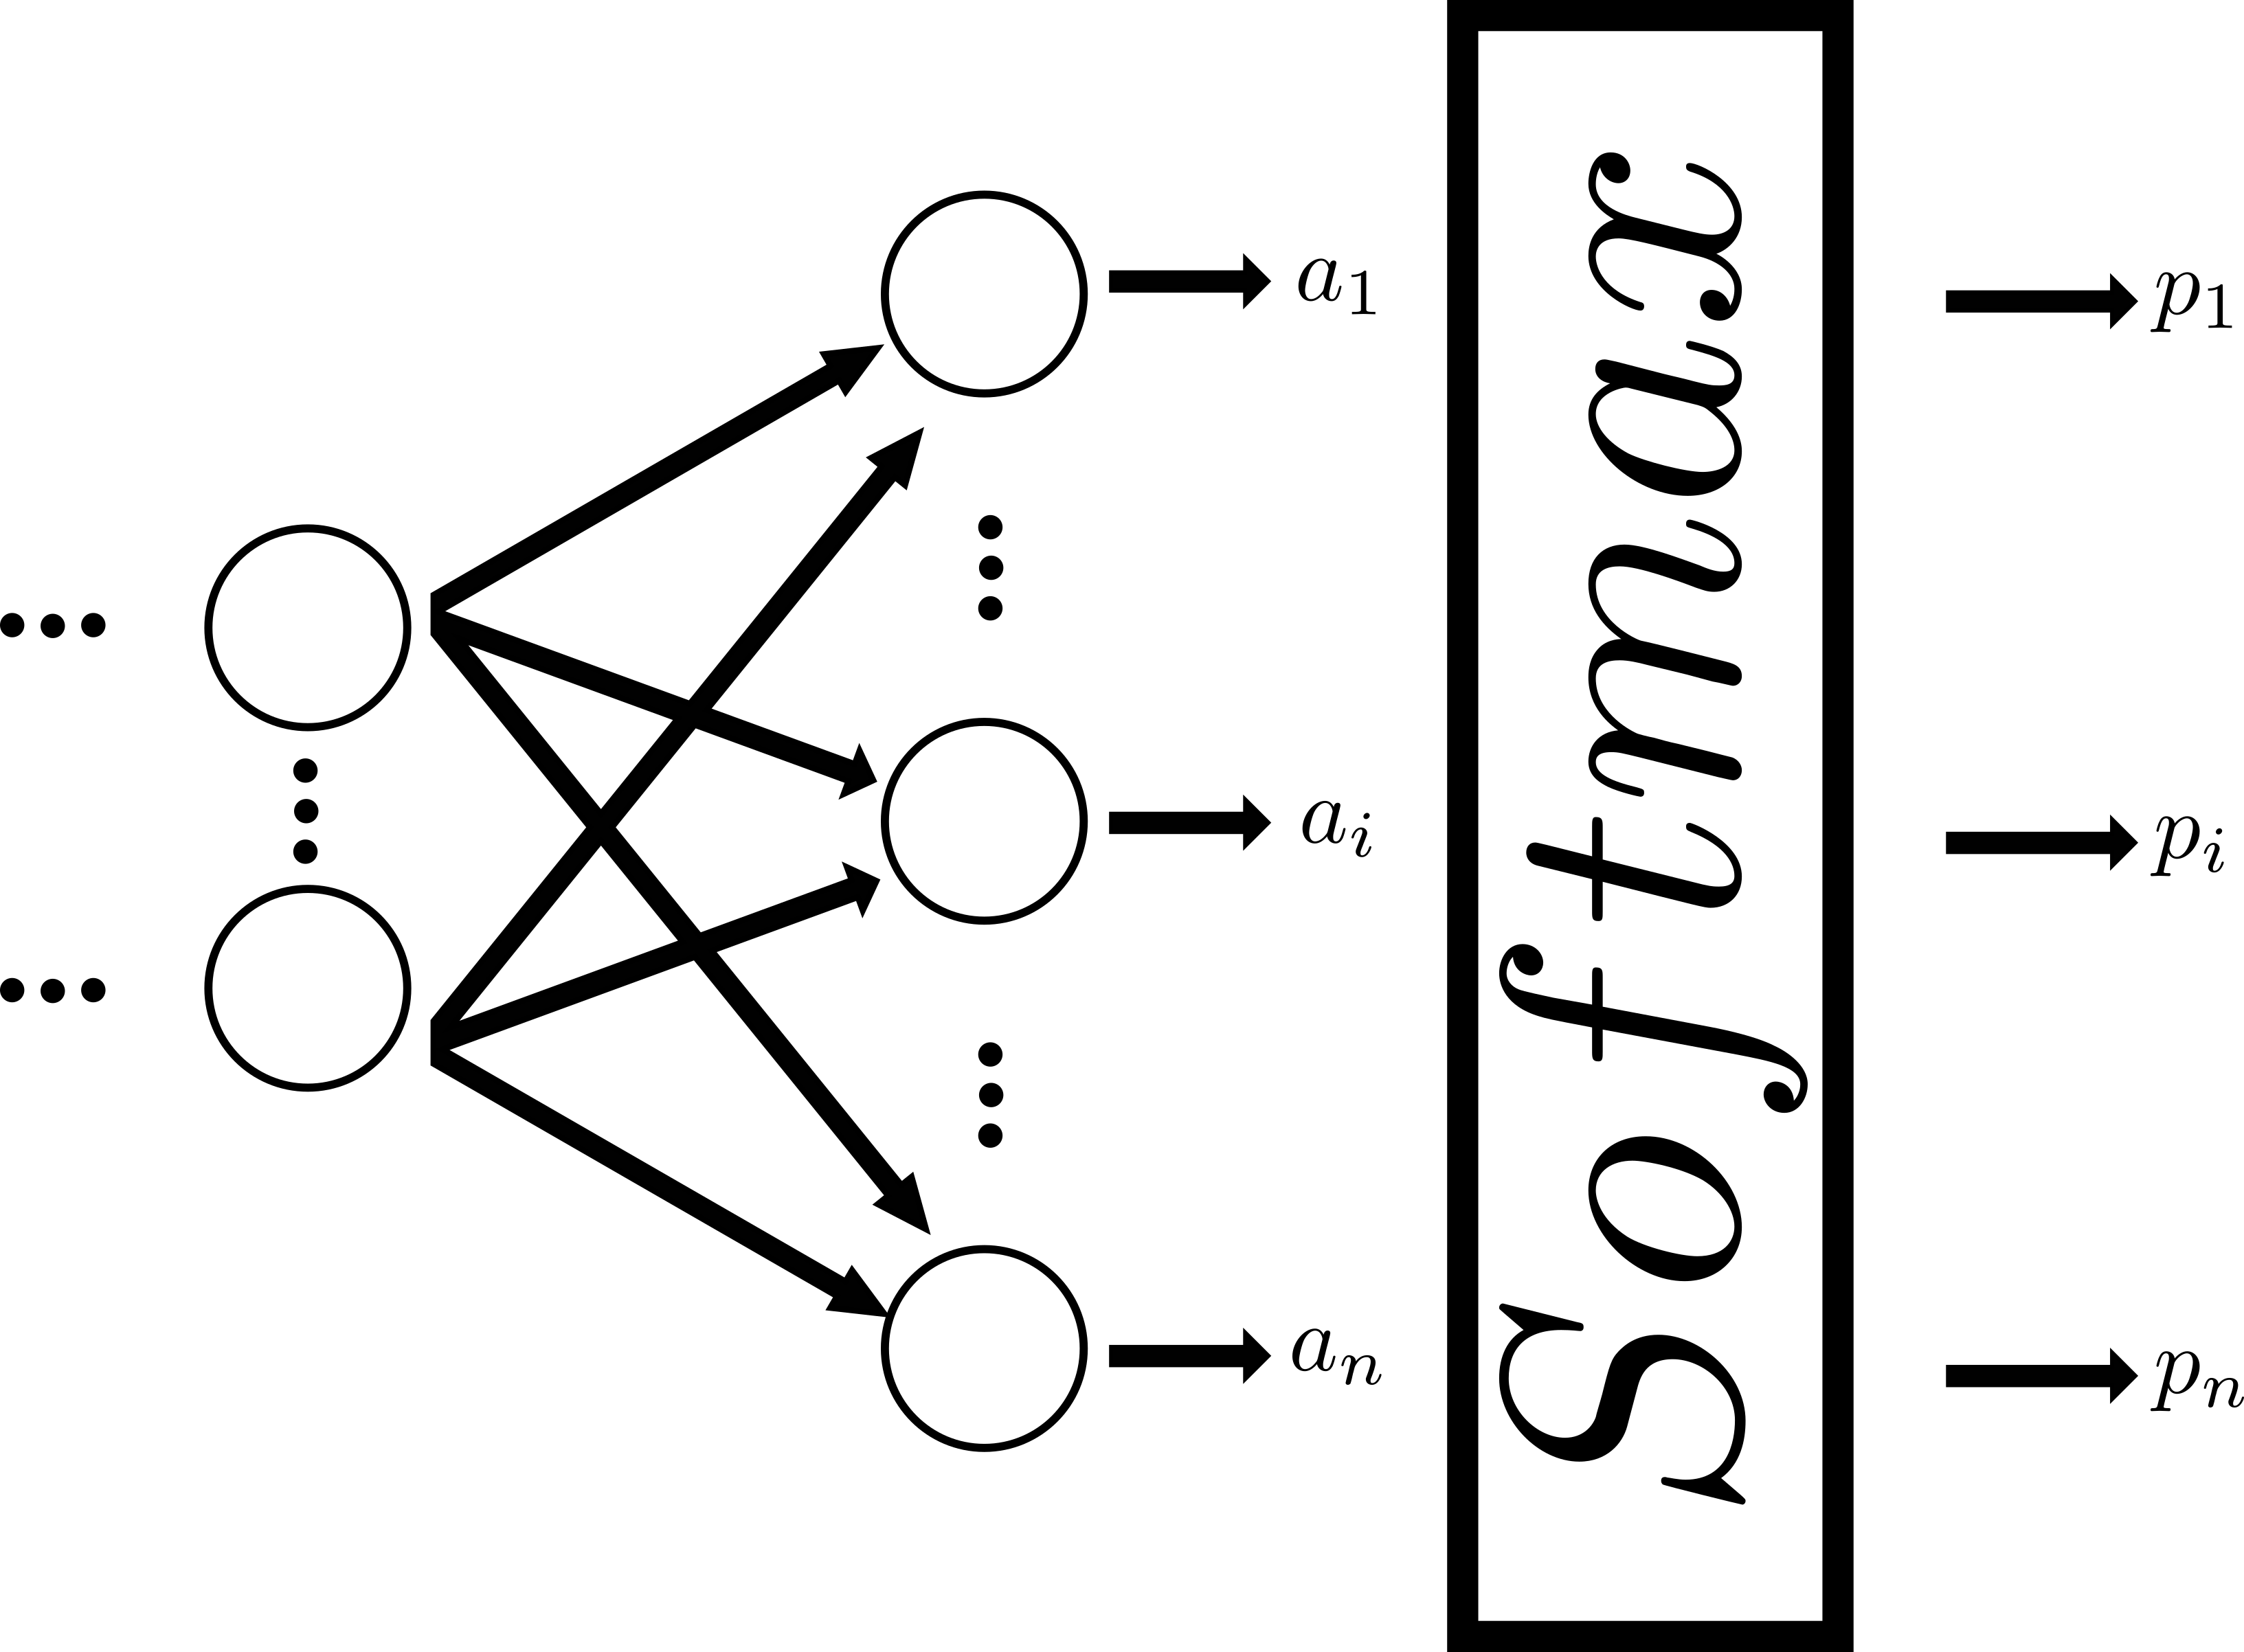
\includegraphics[height=150px]{2-Softmax.png}
		\caption{Schéma d'utilisation du Softmax}
	\end{figure}
\end{frame}


\begin{frame}{V - Mes résultats}
	\begin{columns}[T] % align columns
		\begin{column}{.52\textwidth}
			\begin{figure}
				\centering
				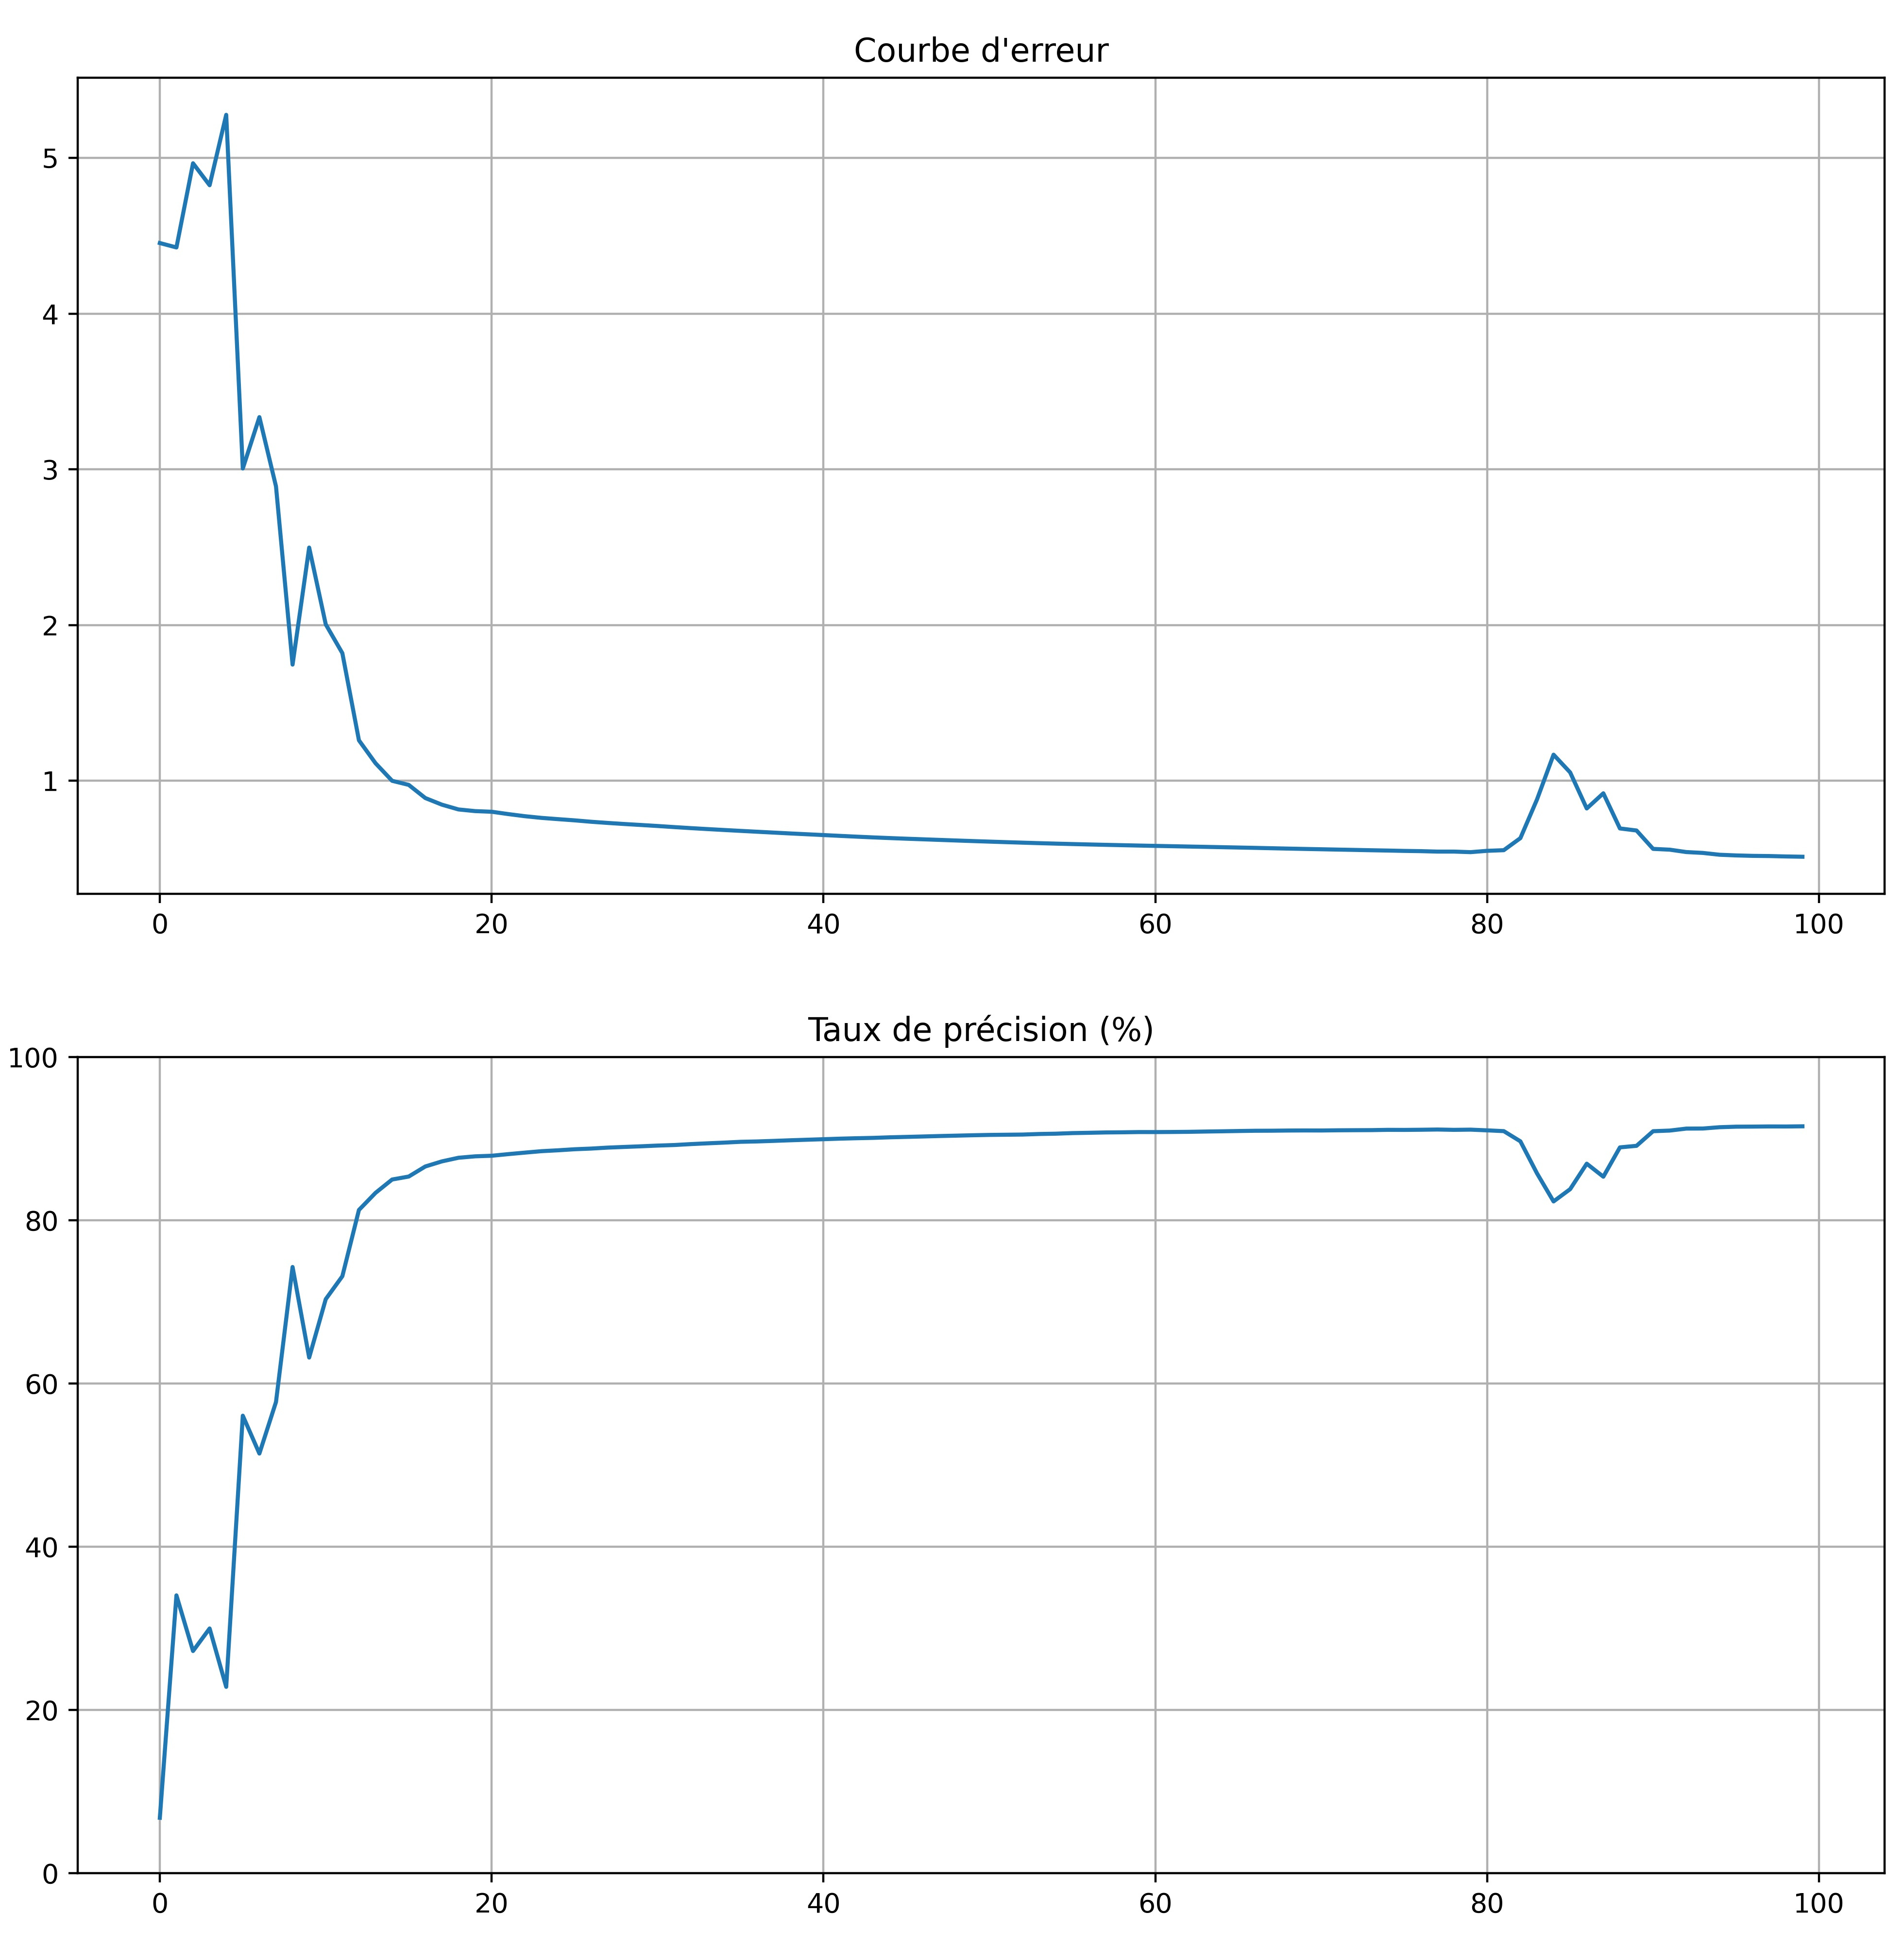
\includegraphics[width=\textwidth]{3-Apprentissage.jpg}
				\caption{Courbes d'apprentissage}
			\end{figure}
		\end{column}
		\hfill
		\begin{column}{.50\textwidth}
			\bigskip	\bigskip	\bigskip
			\bigskip	\bigskip	\bigskip
			\bigskip	\bigskip	\bigskip
			Taux de bonnes réponses après 100 générations d'entrainement : \\
			- 91.5\% sur les données d'entrainement \\
			- 91.3\% sur les données de validation. \\
		\end{column}%
	\end{columns}
\end{frame}


\begin{frame}{V - Mes résultats}
	\begin{figure}
		\centering
		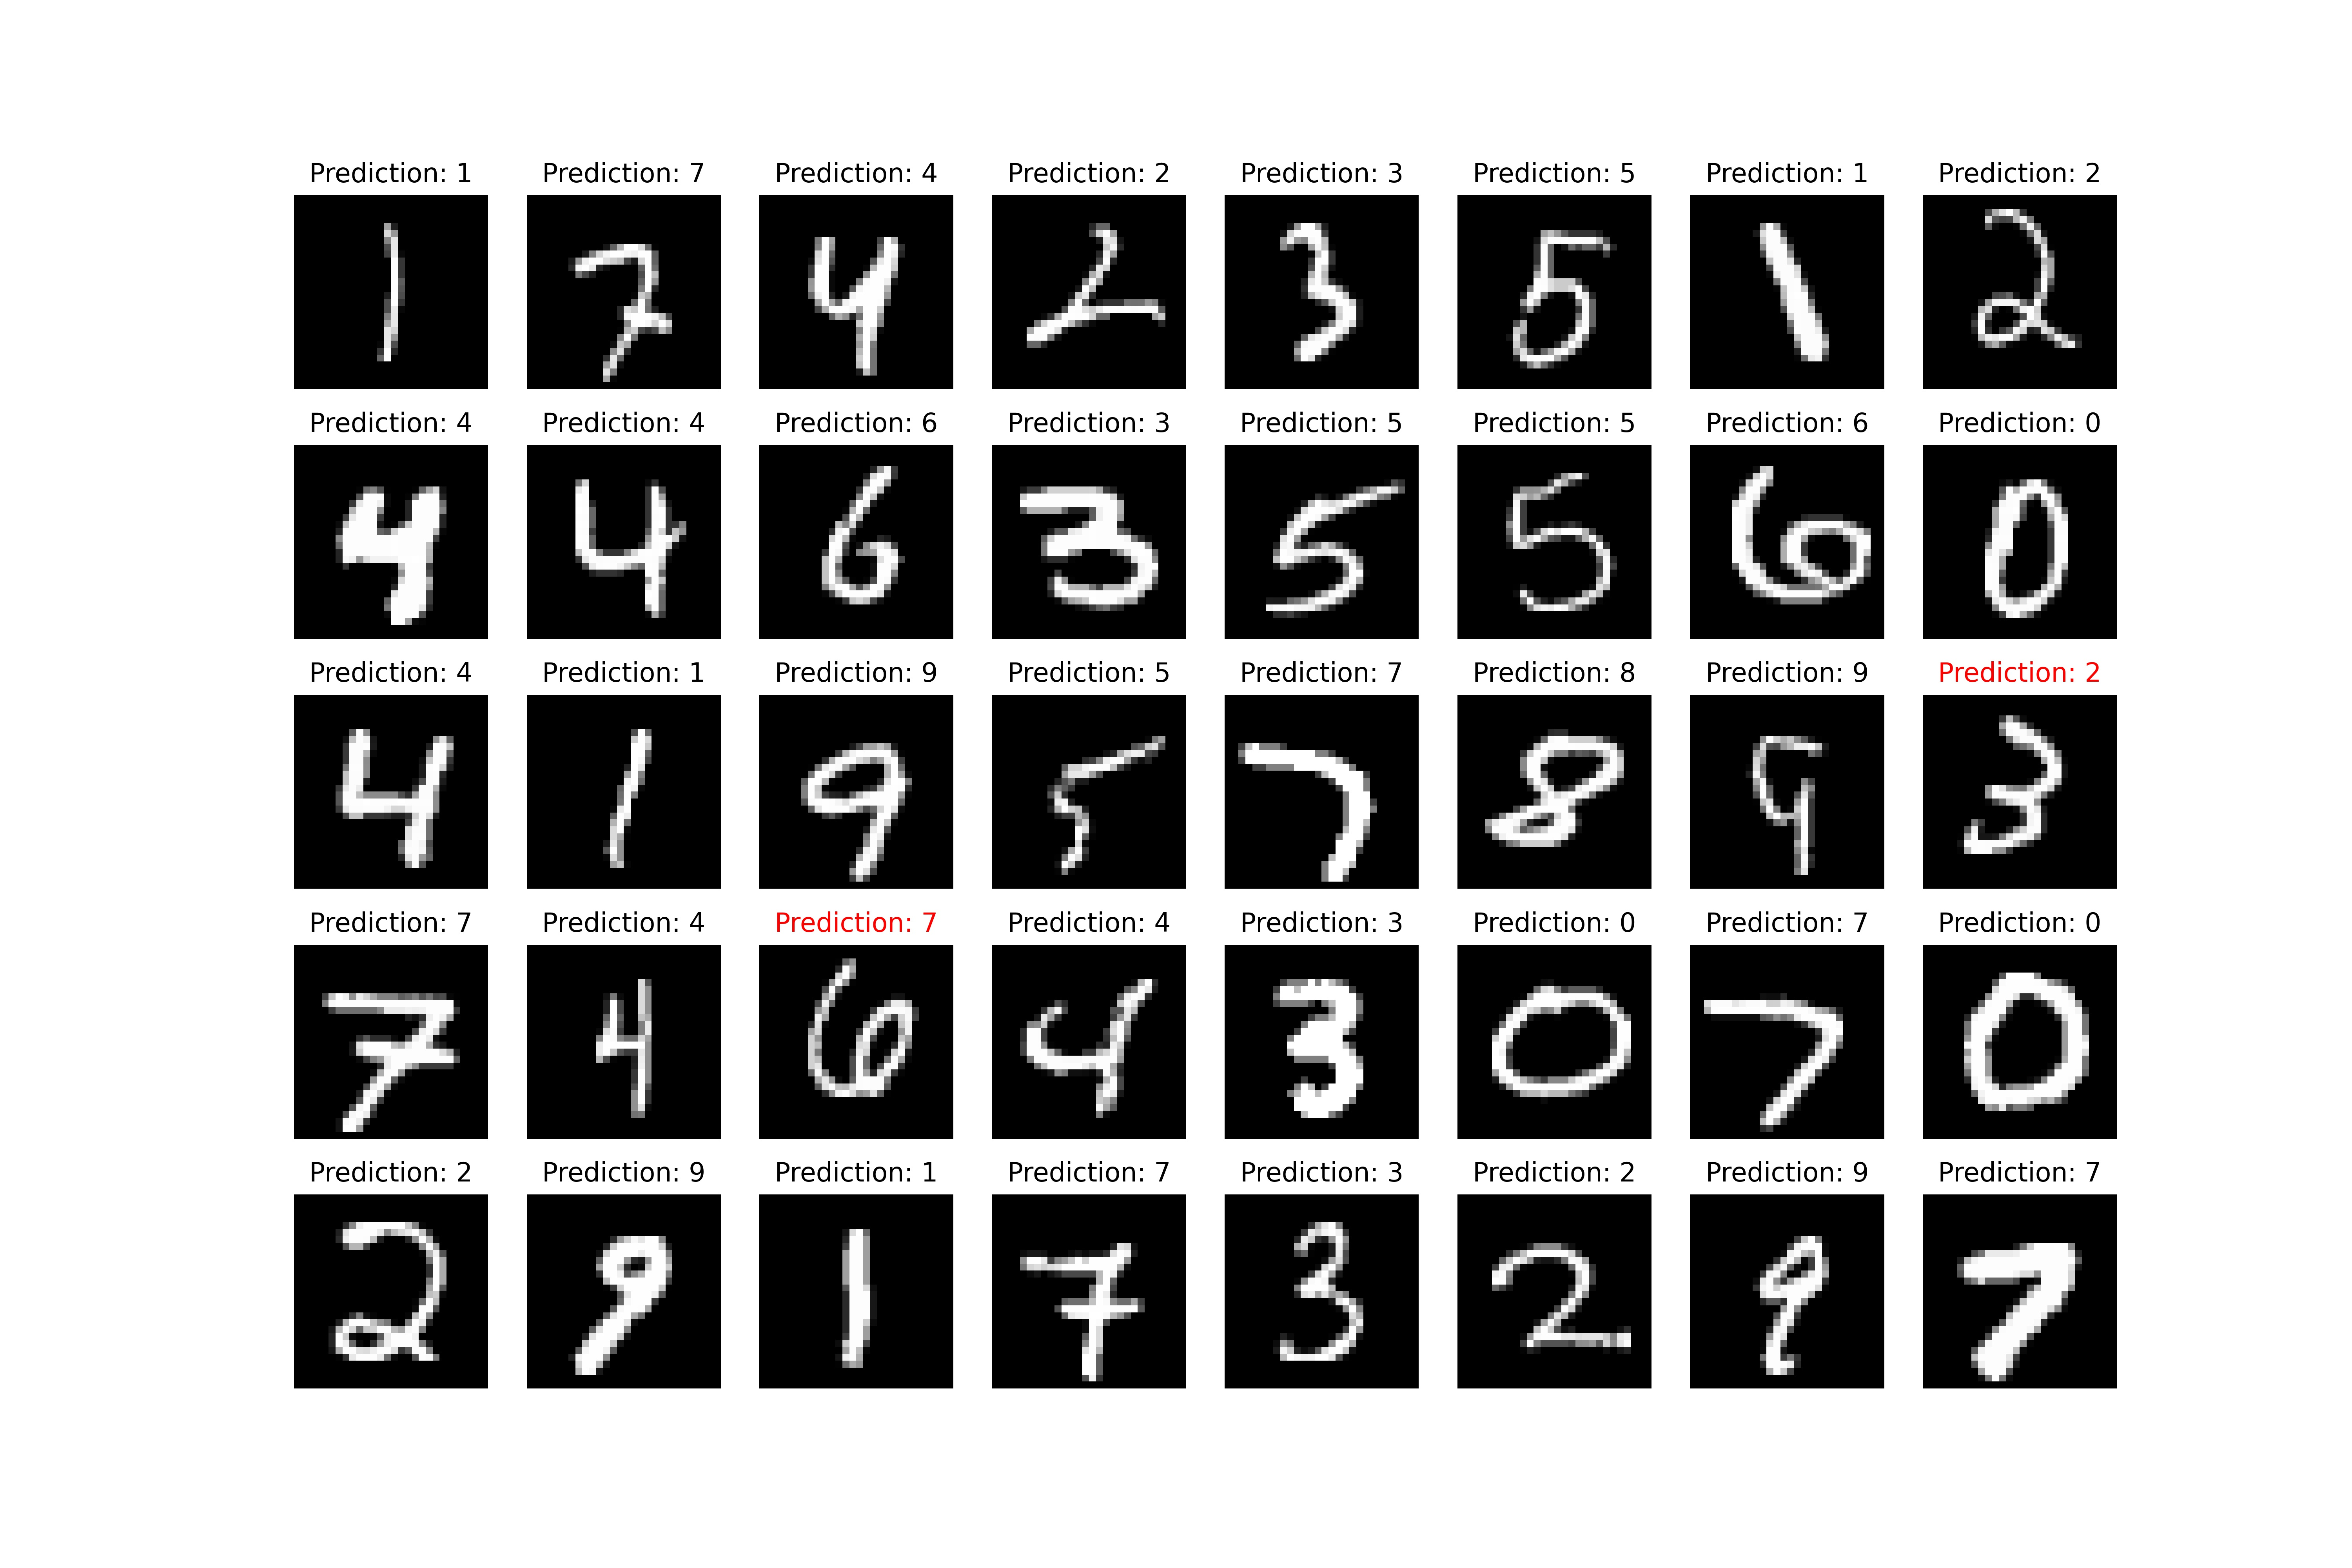
\includegraphics[height=200px]{4-Resultat.jpg}
		\caption{Exemple sur un échantillon de 40 images de validation}
	\end{figure}
\end{frame}


\begin{frame}{V - Convolution d'image}
	\begin{figure}
		\centering
		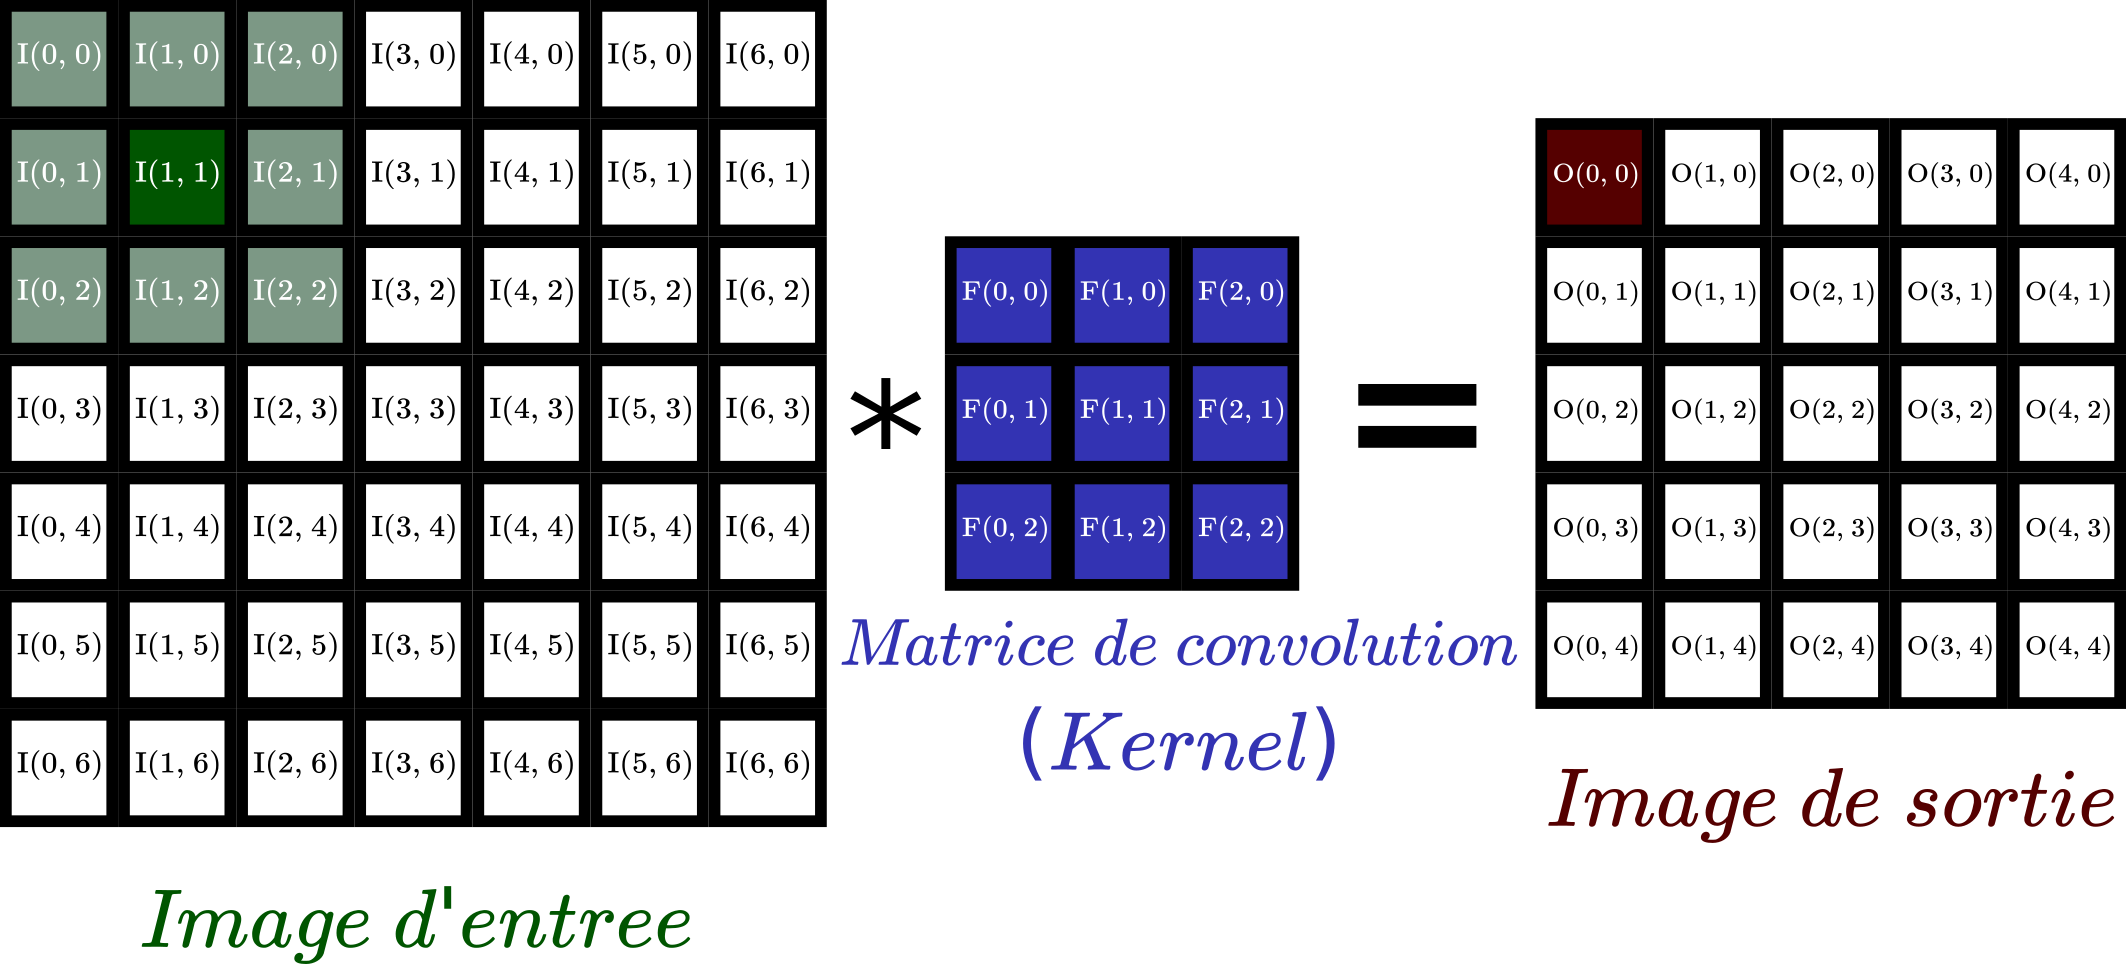
\includegraphics[width=\textwidth]{5-convolution.png}
		\caption{Schéma de la convolution d'image $O(0, 0) = \sum_{i=0}^{2}\sum_{j=0}^{2}I(i, j)\times F(i, j)$}
	\end{figure}
\end{frame}


\begin{frame}{V - Convolution d'image}
	\begin{columns}[T] % align columns
		\begin{column}{.4\textwidth}
			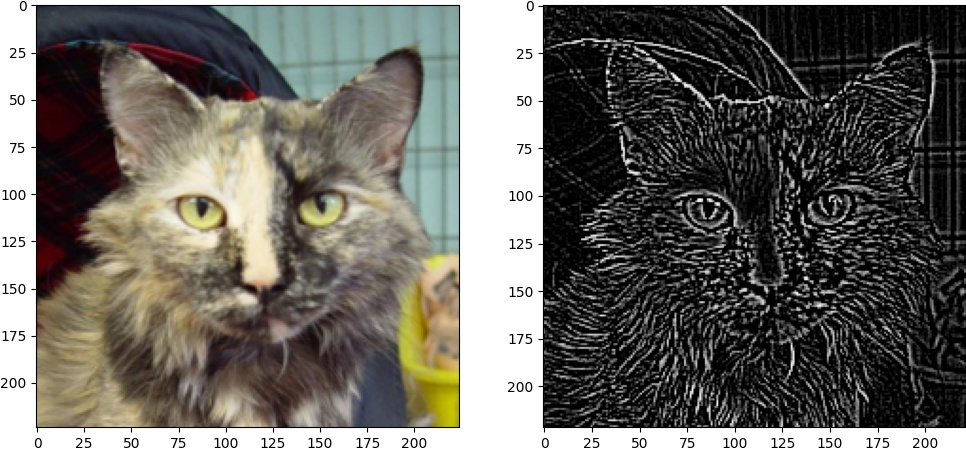
\includegraphics[width=\textwidth]{6-cat.jpg}
			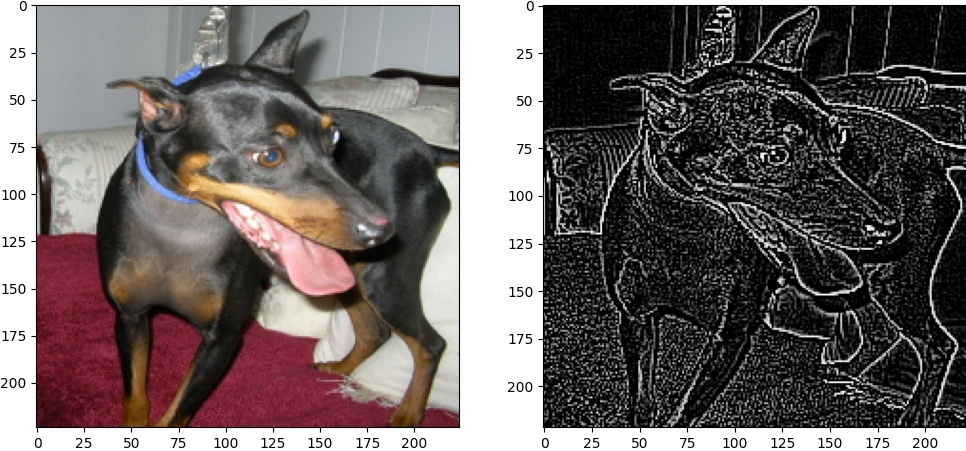
\includegraphics[width=\textwidth]{6-dog.jpg}
			\begin{exampleblock}{Détection de contour}
				\begin{center}
					\centering
					$
					F =
					\begin{pmatrix}
						-1 & -1 & -1 \\
						-1 & 8  & -1 \\
						-1 & -1 & -1
					\end{pmatrix}
					$
				\end{center}
			\end{exampleblock}
		\end{column}
		\hfill
		\begin{column}{.58\textwidth}
			\lstinputlisting[language=Python, firstline=15]{4-convolve.py}
		\end{column}
	\end{columns}
\end{frame}


\begin{frame}{V - Utilisation de réseau de neurones convolutif}
	\begin{columns}[T]
		\begin{column}{.70\textwidth}
			\begin{figure}
				\centering
				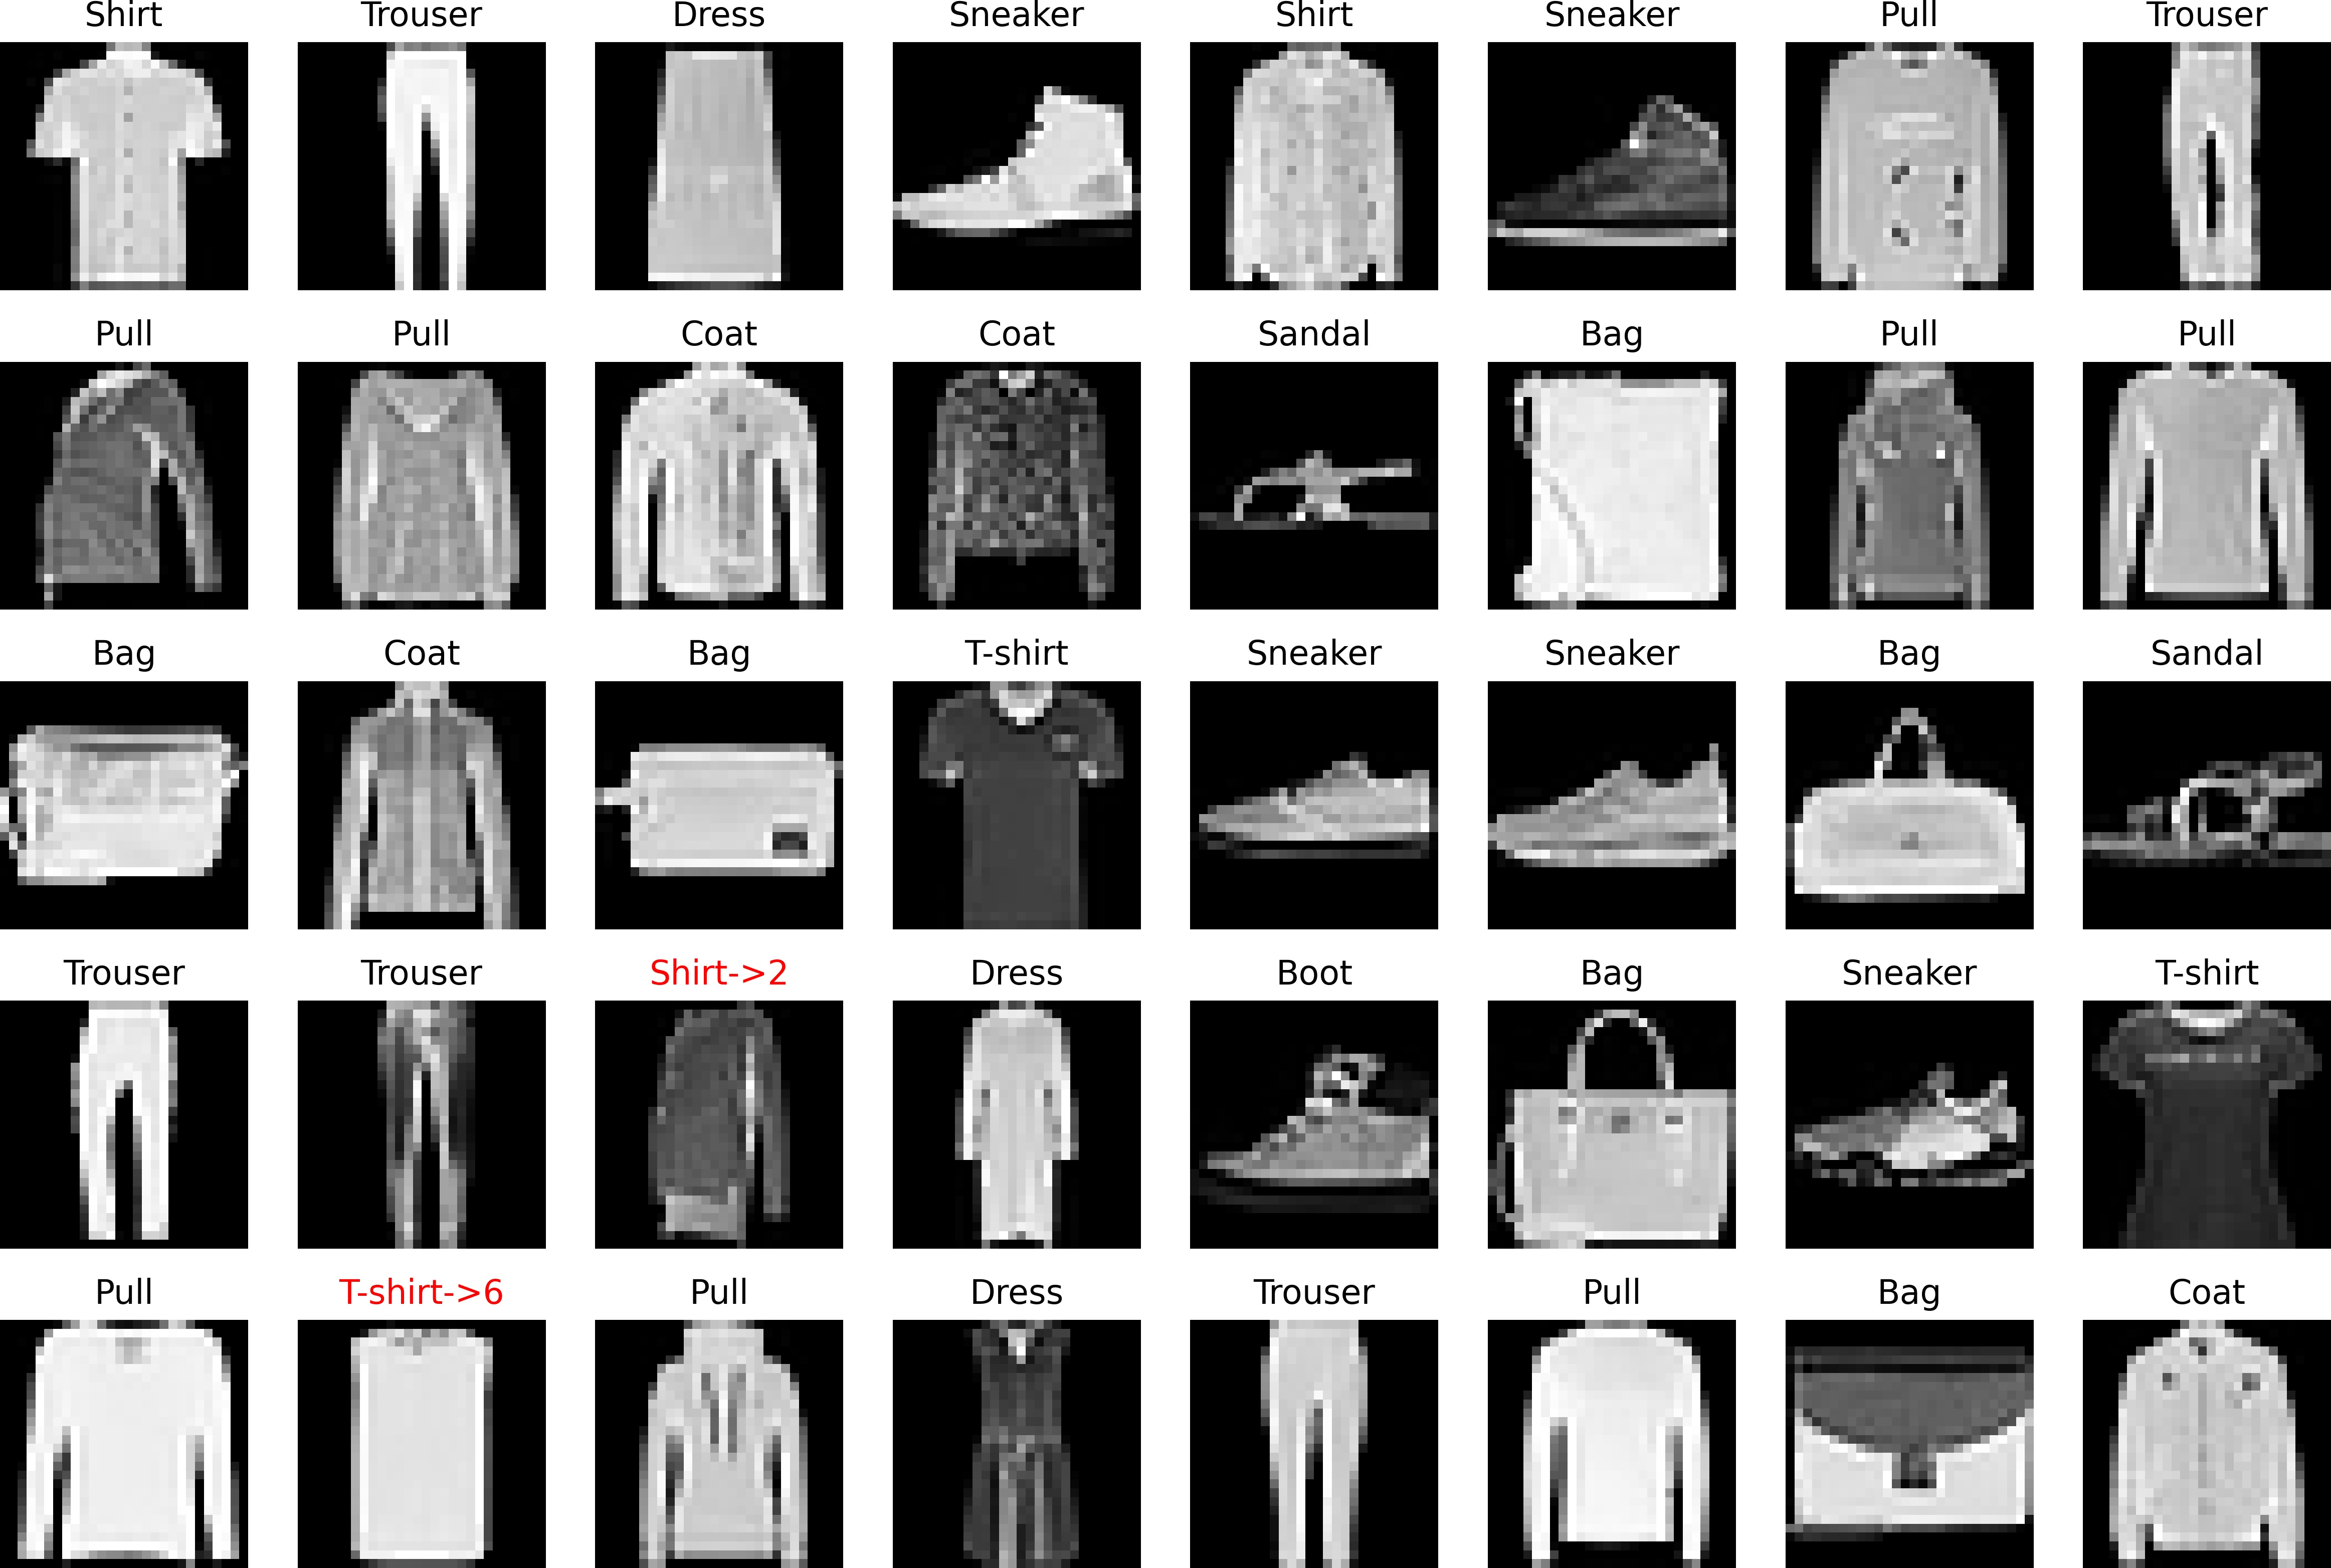
\includegraphics[width=\textwidth]{7-Resultat.jpg}
				\caption{Exemple sur un échantillon de 40 images $Fashion\ MNIST$}
			\end{figure}
		\end{column}
		\hfill
		\begin{column}{.30\textwidth}
			\bigskip	\bigskip	\bigskip
			\lstinputlisting[language=Python, firstline=15]{6-fashionDico.py}
		\end{column}
	\end{columns}
\end{frame}
